\documentclass[aspectratio=169]{beamer}
\usetheme{Madrid}
\usecolortheme{default}
\setbeamertemplate{navigation symbols}{}
\setbeamertemplate{caption}{\insertcaption}
\usepackage{fontspec}
\setmainfont{TeX Gyre Termes}
\usepackage{graphicx}
\usepackage{amsmath,amssymb}
\usepackage{booktabs}
\setbeamerfont{caption}{size=\scriptsize}
\setlength{\parskip}{4pt}

\title{Statistical Analysis of IPL Match Data}
\subtitle{Descriptive Statistics, the Binomial Model, and Regression}
%\author{Group Project}
\institute{Rajagiri College of Social Sciences (Autonomous)}
\date{}

\begin{document}

% ------------------------------------------------------------------ 1 title
\begin{frame}[plain]
\titlepage
\begin{center}
\small A case study on IPL match data from 2008--2018\\[0.7em]
\normalsize\textbf{Group members}\\[0.3em]
Annsteve Jaison \quad $\cdot$ \quad John Jeslin A J \quad $\cdot$ \quad Abhishek Vincent
\end{center}
\end{frame}

% ------------------------------------------------------------------ 2 outline
\begin{frame}{Outline}
\begin{itemize}
\setlength\itemsep{0.6em}
\item Dataset and problem statement
\item Descriptive statistics and visualisation
\item Binomial probability modelling
\item Range-based probabilities
\item Regression: scoring across the decade
\item Conclusions and limitations
\end{itemize}
\end{frame}

% ------------------------------------------------------------------ 3 dataset
\begin{frame}{Dataset and Problem Statement}
\begin{columns}[T]
\column{0.55\textwidth}
\textbf{Source:} supplied IPL match archive, 2008--2018.
\begin{itemize}
\setlength\itemsep{0.35em}
\item 1169 total matches in archive
\item Window 2008--2018 (seasons 1--11): 696 matches
\item 10 removed (no result) $\Rightarrow$ \textbf{686 decided matches}
\item 10 of 19 variables retained
\end{itemize}
\vspace{0.25em}
\textbf{Objectives}
\small
\begin{enumerate}
\setlength\itemsep{0.1em}
\item Summarise matches (central tendency, dispersion)
\item Model the win process with the Binomial distribution
\item Compute range-based probabilities
\item Test for a scoring trend with linear regression
\end{enumerate}
\normalsize

\column{0.45\textwidth}
\centering
\small \textbf{Selected variables}
\begin{tabular}{ll}
\toprule
Variable & Role\\
\midrule
season & time index\\
toss\_decision & bat / field\\
winner & outcome\\
result & runs / wickets / tie\\
result\_margin & margin\\
target\_runs & first-innings score\\
\bottomrule
\end{tabular}
\end{columns}
\end{frame}

% ------------------------------------------------------------------ 4 descriptive
\begin{frame}{Descriptive Statistics}
\begin{columns}[T]
\column{0.5\textwidth}
\textbf{Target runs} (n = 686)\\
Mean 161, median 163, mode 166\\
SD 32.4 \quad CV 0.20\\[0.4em]
\textbf{Victory margin} (n = 685)\\
Mean 17, median 8\\
SD 22.0 \quad CV 1.29\\[0.4em]
Margins are strongly right-skewed (skew 2.8):\\
most games are close, blow-outs are rare --- yet the
maximum reaches 146 runs.

\column{0.5\textwidth}
\centering
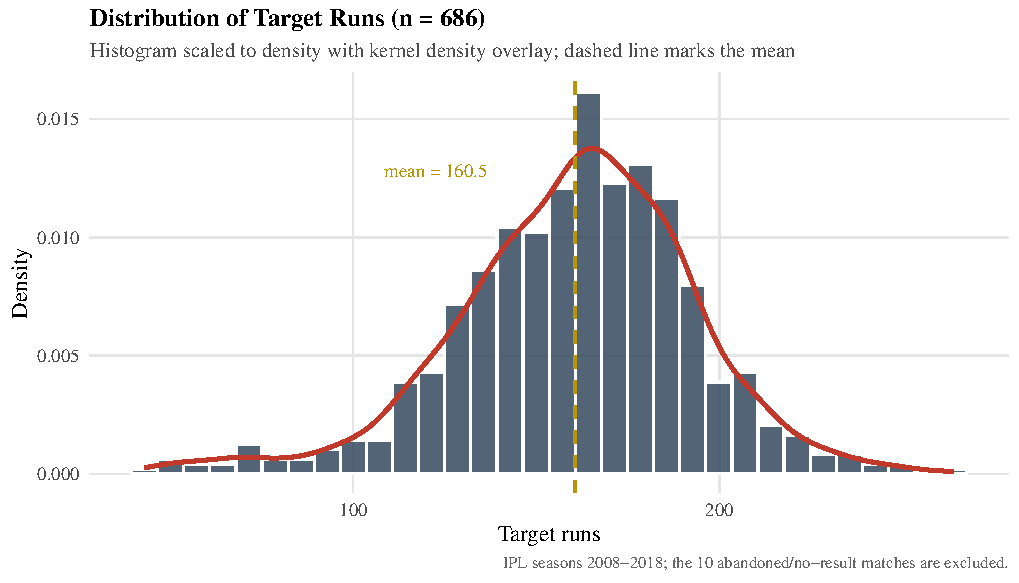
\includegraphics[width=\textwidth]{figures/fig_target_hist.pdf}
\end{columns}
\end{frame}

% ------------------------------------------------------------------ 5 boxplot
\begin{frame}{Dispersion: Box-and-Whisker Comparison}
\begin{center}
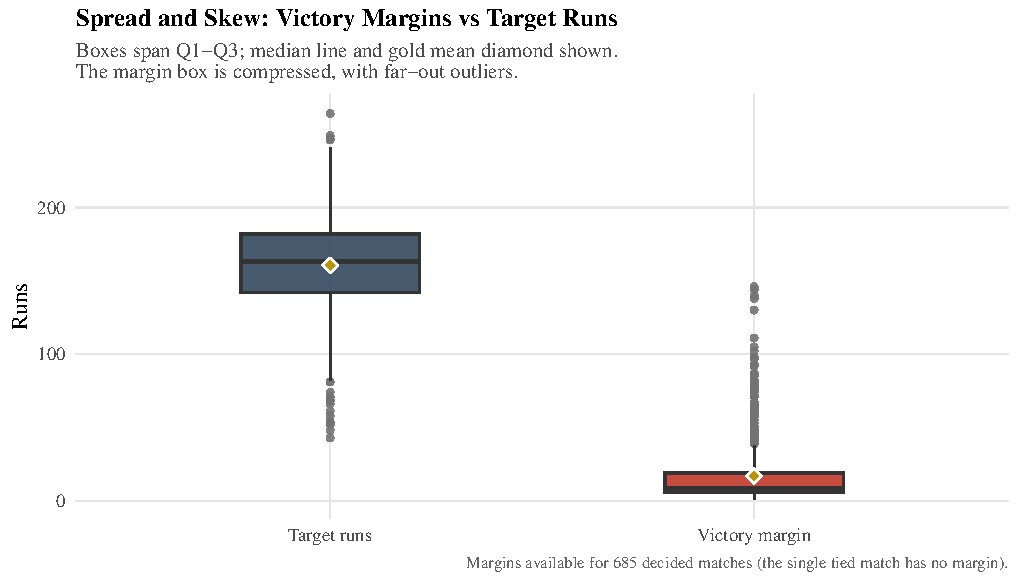
\includegraphics[width=0.8\textwidth]{figures/fig_boxplots.pdf}
\end{center}
\begin{itemize}
\item Targets: tight cluster around 160--165 (IQR 40)
\item Margins: compressed box, long whisker to 146 $\Rightarrow$ right skew
\end{itemize}
\end{frame}

% ------------------------------------------------------------------ 6 binomial
\begin{frame}{The Binomial Model: First-Innings Advantage}
Each match is a Bernoulli trial with $p = $ win probability; counts follow
$X \sim \text{Binomial}(n,p)$.

\begin{center}
\begin{tabular}{lccl}
\toprule
Strategy & wins / n & $\hat{p}$ & $p$-value (H$_0$: $p=0.5$)\\
\midrule
Bat first & 128 / 279 & 0.459 & 0.188\\
Chase & 226 / 407 & \textbf{0.555} & \textbf{0.029}\\
\bottomrule
\end{tabular}
\end{center}

\vspace{0.8em}
Chasing estimate is \textbf{significantly} above 0.5 ($p=$ 0.029):\\
a real, modest advantage for the fielding side this decade.
\end{frame}

% ------------------------------------------------------------------ 7 binomial ci
\begin{frame}{Binomial Estimates with 95\% Confidence Intervals}
\begin{center}
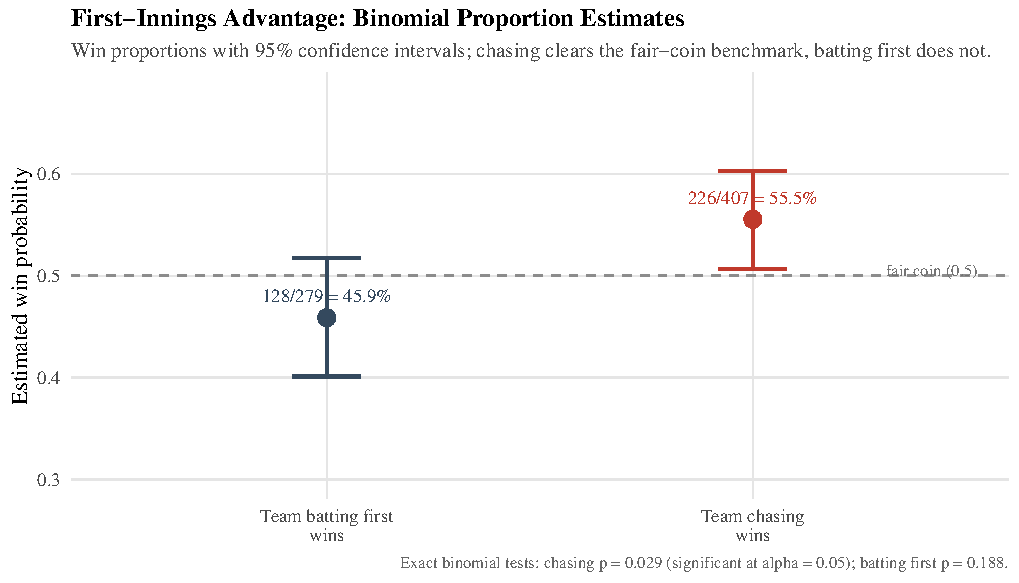
\includegraphics[width=0.70\textwidth]{figures/fig_binomial_ci.pdf}
\end{center}
\vspace{-0.2em}
The chasing interval lies entirely above the fair-coin line (0.5);
the batting-first interval straddles it.
\end{frame}

% ------------------------------------------------------------------ 8 pmf
\begin{frame}{Probability Mass Function of Wicket Margins}
\begin{columns}[T]
\column{0.5\textwidth}
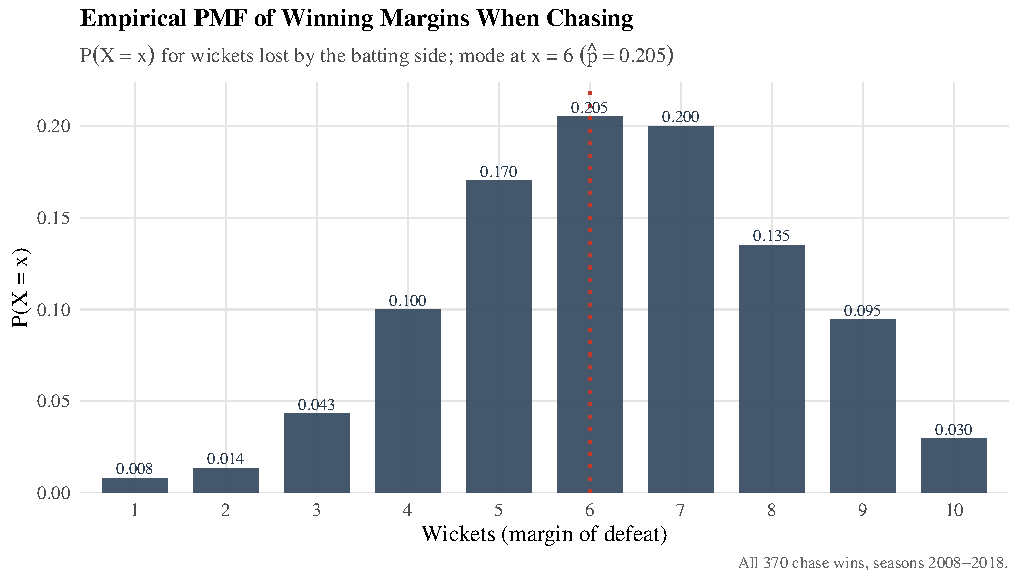
\includegraphics[width=\textwidth]{figures/fig_pmf_wickets.pdf}
\column{0.5\textwidth}
When a chase succeeds, the margin is \emph{wickets in hand}, a discrete
variable $X \in \{1,\dots,10\}$.

\begin{itemize}
\setlength\itemsep{0.5em}
\item Mode at $X=6$: $P(X=6)=0.205$
\item Unimodal, concentrated between 3--8
\item Rare to win by 1 or 10 wickets
\end{itemize}
\end{columns}
\end{frame}

% ------------------------------------------------------------------ 9 range probs
\begin{frame}{Range-Based Probabilities}
Where closed-form integrals are not available, probabilities are estimated by
relative frequency:
\begin{center}
\begin{tabular}{lcc}
\toprule
Event & Estimate\\
\midrule
$P(140 \le T \le 160)$ & 0.233\\
$P(161 \le T \le 190)$ & 0.389\\
$P(T > 200)$ & 0.087\\
$P(T < 120)$ & 0.093\\
$P(\text{margin} > 50)$ & 0.074\\
\bottomrule
\end{tabular}
\end{center}
Most targets fall in the 140--190 band; scores above 200 are uncommon.
\end{frame}

% ------------------------------------------------------------------ 10 regression
\begin{frame}{Regression: Scoring Across the Decade}
\begin{columns}[T]
\column{0.5\textwidth}
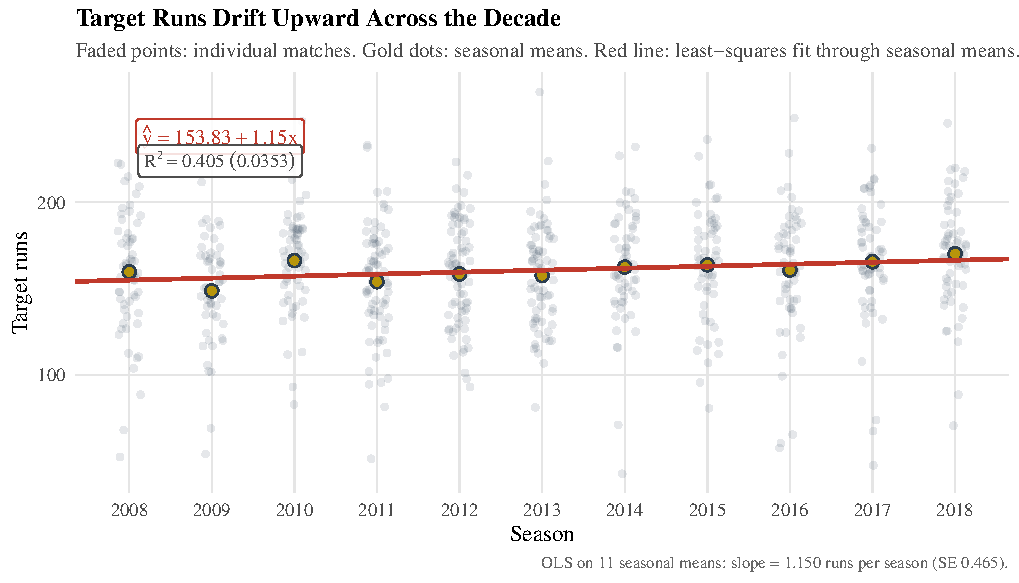
\includegraphics[width=\textwidth]{figures/fig_regression.pdf}
\column{0.5\textwidth}
Least-squares fit on 11 seasonal means:
$$\hat{y} = 153.9 + 1.15\,x$$
\begin{itemize}
\setlength\itemsep{0.5em}
\item Slope +1.15 runs/season
\item $R^2 = 0.405$
\item $p = 0.035$ (significant at 5\%)
\end{itemize}
\vspace{0.5em}
First-innings targets drifted \emph{upward} across 2008--2018.
\end{columns}
\end{frame}

% ------------------------------------------------------------------ 11 conclusion
\begin{frame}{Conclusions}
\begin{itemize}
\setlength\itemsep{0.7em}
\item Targets concentrate near 160--165 and rise $\approx$1.2 runs/season
\item Margins are heavily right-skewed --- T20 is a game of close finishes
\item \textbf{Chasing wins more often than not} ($\hat p=0.555$, $p=0.029$)
\item Toss alone is still a coin flip (no inherent luck)
\item Team dominance is real but measured (CSK 90/146, $p=0.006$)
\end{itemize}
\end{frame}

% ------------------------------------------------------------------ 12 limitations
\begin{frame}{Limitations \& Reflection}
\begin{itemize}
\setlength\itemsep{0.7em}
\item Relative-frequency estimates assume a representative sample;
  conclusions describe the 2008--2018 era, not cricket in general
\item Ten variables collapse rich covariates (venue, opponents, pitch)
\item A venue/opponent-aware model would refine the estimates
\item Techniques map directly to the curriculum: PMF, Binomial, range
  probabilities, regression
\end{itemize}
\vspace{0.6em}
\begin{center}
\emph{Thank you.}
\end{center}
\end{frame}

\end{document}
